{\large\section*{Теоритические вопросы}}

\begin{enumerate}
	\item \textit{Какое первое состояние резольвенты?}
	
	\qquad \textbf{Ответ}: первое состояние резольвенты представляет собой вопрос.

	\item \textit{В каком случае система запускает алгоритм унификации? (Как эту необходимость на формальном уровне распознает система?)}

	\qquad \textbf{Ответ}: алгоритм унификации запускается системой в случае необходимости проверить, подходит ли текущее правило в базе знаний для доказательства текущей цели.

	\item \textit{Каковы назначение и результат использования алгоритма унификации?}
	
	\qquad \textbf{Ответ}: результат алгоритма унификации представляет ответ да или нет. При ответе да результатом также является подстановка, сформированная в процессе работы алгоритма.
	
	\item \textit{В каких пределах программы уникальны переменные?}
	
	\qquad \textbf{Ответ}: именованные переменные уникальны в пределах предложения, а анонимные переменные уникальны всегда.

	\item \textit{Как применяется подстановка, полученная с помощью алгоритма унификации?}
	
	\qquad \textbf{Ответ}: все переменные, содержащиеся в постановке и в термах резольвенты, заменяются в резольвенте на соответствующие значения для этих переменных.

	\item \textit{Как меняется резольвента?}
	
	\qquad \textbf{Ответ}: при нахождении похдодящего правила для первого терма резольвенты он заменяется на тело правила.
	
	\item \textit{В каких случаях запускается механизм отката?}

	\qquad \textbf{Ответ}: механизм отката запускается в случае, когда система попадает в тупиковое состояние -- резольвента не пуста, но вся база знаний уже была просмотрена с целью подбора знания для текущей цели доказательства.
\end{enumerate}

{\large\section*{Задание}}

В одной программе написать правила, позволяющие найти:

\begin{enumerate}[1.]
	\item максимум из двух чисел (с/без использования отсечения);
	\item максимум из трех чисел (с/без использования отсечения).
\end{enumerate}

Убедиться в правильности результатов.

Для каждого случая пункта 2 обосновать необходимость всех условий тела. Для одного из вариантов ВОПРОСА и каждого варианта задания 2 составить таблицу, отражающую конкретный порядок работы системы.

\clearpage

{\large\section*{Текст программы}}

\begin{lstlisting}
domains
	num = integer
	numList = integer*

predicates
	max(num, num, num).
	max(num, num, num, num).
	max(num, numList).

clauses
	max(A, A, B) :- A >= B.
	max(B, _, B).
	
	max(A, A, B, C) :- A >= B, A >= C.
	max(B, _, B, C) :- B >= C.
	max(C, _, _, C).
	
	max(A, [A]) :- !.
	max(A, [A, B]) :- A >= B, !.
	max(B, [_, B]) :- !.
	max(R, [A|T]) :- max(R1, T), max(R, A, R1).

goal
	max(R, [1, 3, 5, 2, 7, 0]).
\end{lstlisting}

\clearpage

{\large\section*{Порядок поиска ответа для вопросов}}

Порядок поиска ответа для 1 варианта:

\vspace*{5mm}

\begin{center}
	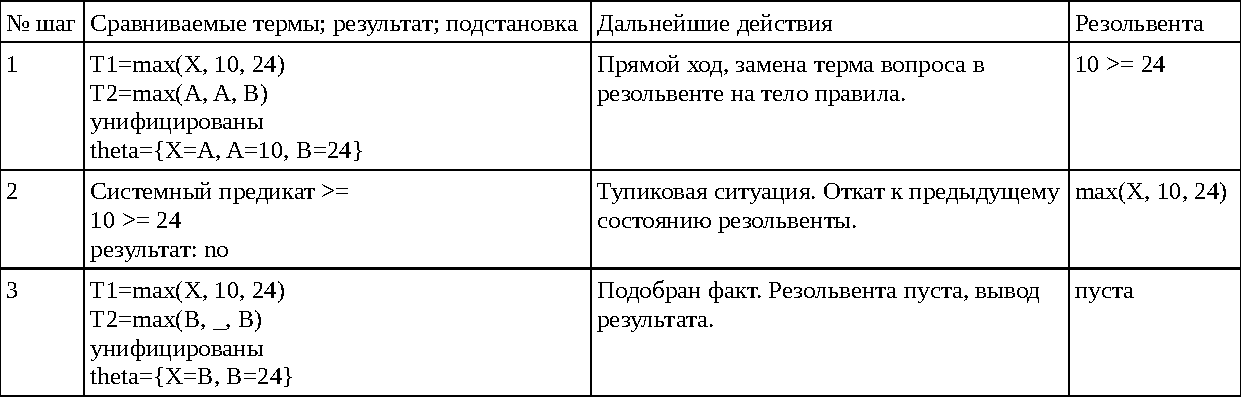
\includegraphics[width=\linewidth]{table1.pdf}
\end{center}

Порядок поиска ответа для 2 варианта:

\begin{center}
	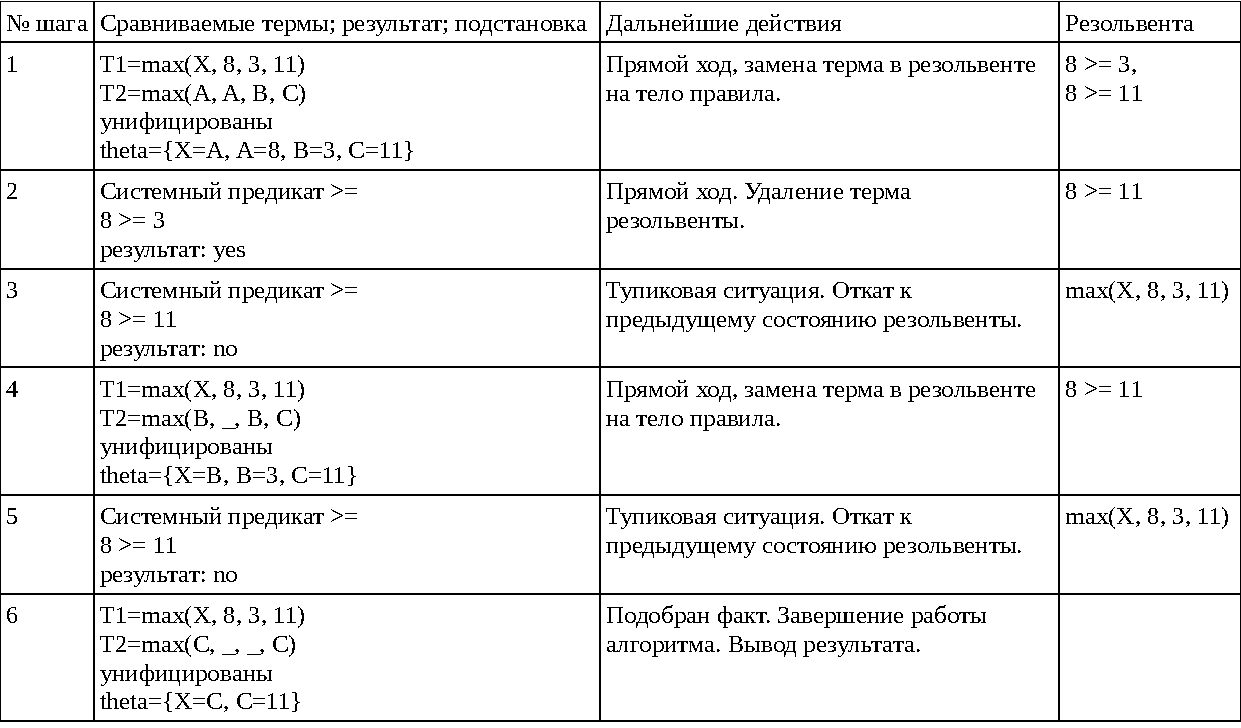
\includegraphics[width=\linewidth]{table2.pdf}
\end{center}
